% -------------------------------------------------------------------------------------------------
% figure ----
% -------------------------------------------------------------------------------------------------
\begin{figure}[t!]\hfill
    \begin{subfigure}{.5\textwidth}\centering
        \caption{Factor Loadings before rotation}
        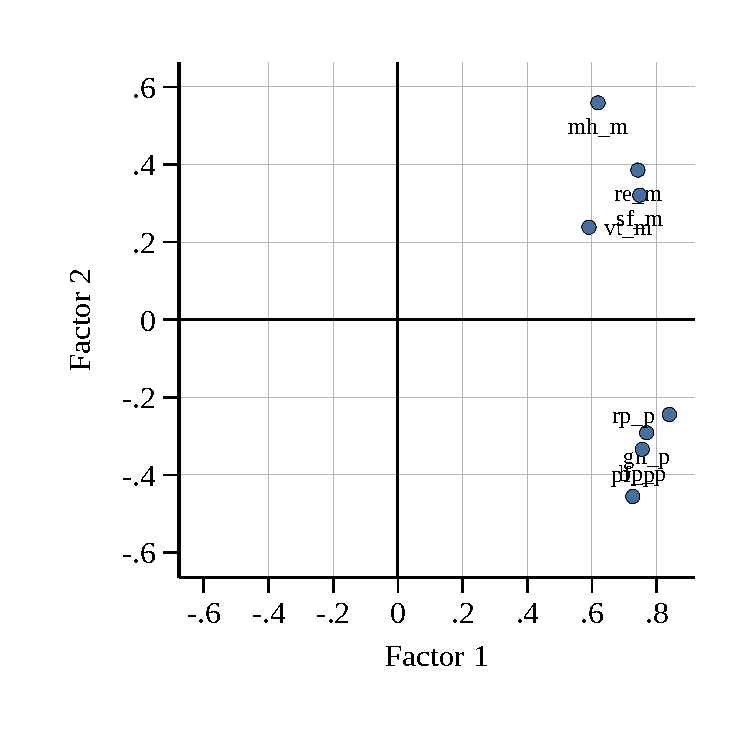
\includegraphics[width=.9\linewidth]{../../output/figures/factor/factor_loadings_norotate.pdf}
        \label{sfig:factorloadingsnorotate}
    \end{subfigure}\\
    \begin{subfigure}{.5\textwidth}\centering
        \caption{SOEP's default (SF-12)\\PCA followed by varimax rotation\\(with Kaiser normalization)}
        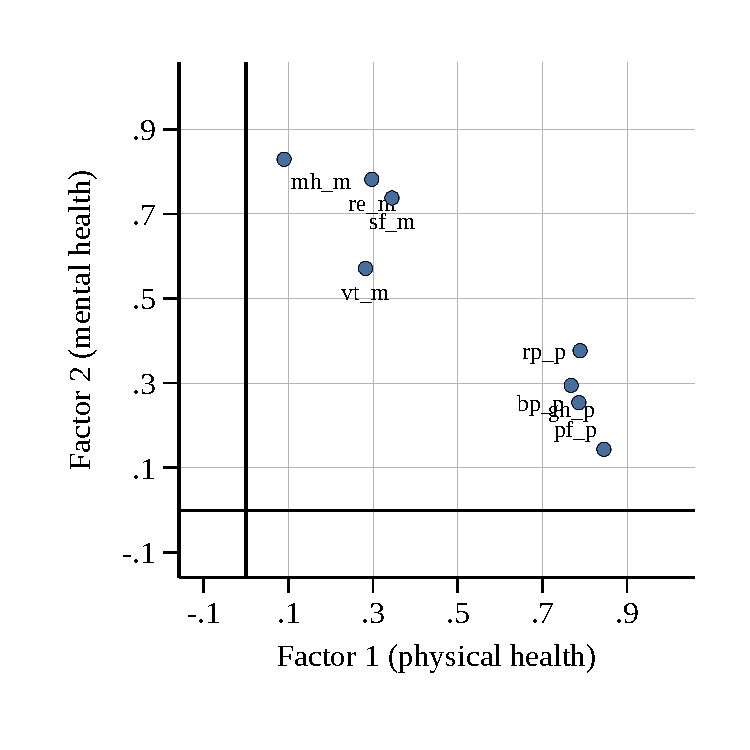
\includegraphics[width=.9\linewidth]{../../output/figures/factor/factor_loadings_a_soeps_default.pdf}
        \label{sfig:factorloadingsdef}
    \end{subfigure}%
    \begin{subfigure}{.5\textwidth}\centering
        \caption{Alternative method\\Principal factors with oblique rotation\\(promax=1.6)}
        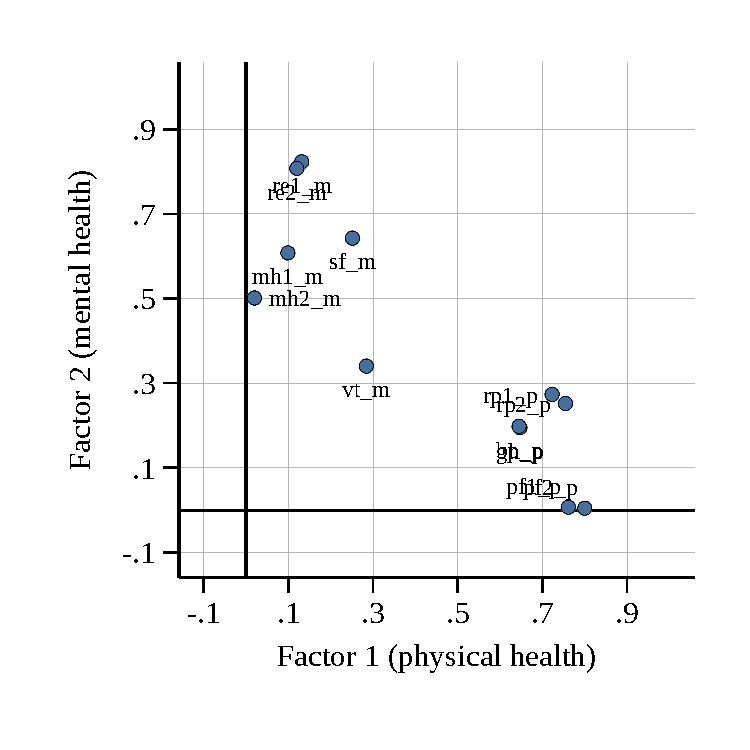
\includegraphics[width=.9\linewidth]{../../output/figures/factor/factor_loadings_b_oblique_main_raw_input_vars.pdf}
        \label{sfig:factorloadingmain}
    \end{subfigure}%
    \caption[Factor loadings comparison between SF-12 and alternative methods]
    {Factor loadings comparison between SF-12 and alternative methods} 
    \label{fig:factorloadings}
    \fnote{
    Notes: The graphs show in both versions that the variables are meaningfully clustered in their
    respective group and the clusters are well separated. However, allowing for an oblique rotation
    results in a clearer factor separation. The loadings of each variable are closer to one of the
    axes, indicating that a variable strongly affects one but not the other factor. 
    Further, by using all variables instead of the mean of grouped variables in the alternative model
    we can confirm that variables from the same category are indeed closely clustered. One drawback
    with the alternative model is that \code{vt} (Vitality) is only weakly loaded from both factors.
    Variables with suffix \textit{m} belong to the mental domain, whereas those with \textit{p} to the physical one. 
    For an overview on the variables see \cref{tab:health_fact_varname_and_questions}. 
    }
\end{figure}